\documentclass[main.tex]{subfiles}
\begin{document}

\newpage
\chapter{FLUKA Results}

The following results chapter focuses on the analysis of the calculations using the copper target configuration without shielding (\textbf{cp\_OOOO}). The same tables and plots for the other facility configurations can be found in the appendix. All results tables can also be found at \url{http://thornton.web.cern.ch/fluka_data.html}  \\

There are two different types of information at the test positions that can be taken from the results of the simulations. The first is the integral values: dose or particle fluence at that specific location for example. These are useful for simple tests relating to subjects such as tolerance to dose or certain particle types. The second is the fluence of different particles with respect to energy (spectral information) for each of the test positions. This can be used to explore effects correlated with energy, for example the effect of high energy particles on the response of the detector by placing in positions of low and high average particle energy (such as the hardness factor, mentioned in the previous chapter). \\

In terms of HEH fluence, it is possible to emulate many different radiation environments within the CHARM test area. The plot in figure \ref{fig:example_rev_spectra} shows the reverse integral spectra for several radiation environments compared to those at different test positions, marked in grey. A table of the hardness factors for different environments are given in figure \ref{tab:hardness_energies} [reference]. The values for the 10\% (H10) and 50\% (H50) hardness factors can be found in tables \ref{tab:hardness50} and \ref{tab:hardness50} respectively. \\

\begin{figure}[ht]
	\centering
	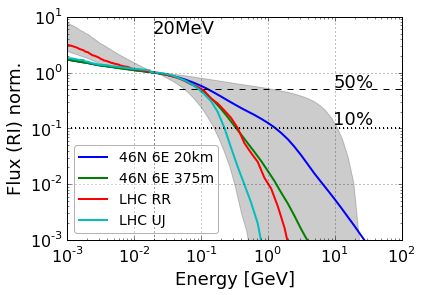
\includegraphics[scale=0.6]{./images/rev_spectra_example}
	\caption{A plot of the reverse integral spectra for test positions at CHARM (in grey), compared with different radiation environments, normalised to 20 MeV.}
	\label{fig:example_rev_spectra}
\end{figure}

\begin{table}[htbp]
  \sisetup{tight-spacing=true}
  \centering
    \begin{tabular}{l|c|c}
	Environment & Rack & Acc. Factor \\
	\hline
	\hline
	375m		& 9		& 1.4E8 \\
	20km		& 16	& 1.2E6 \\
	Proba-II	& 7		& 8.1E3 \\
	LHC HS		& 3		& 7.0E3 \\
	LHC LS		& 14	& 3.3E4 \\
	LHC Tunnel	& 19	& 60 \\
	LHC Exp. 	& - 	& - \\
    \end{tabular}
	\caption{A table showing the matches and respective acceleration factors for the CP\_OOOO configuration with different environments. For the LHC experimental areas, a match may be found with an alternative configuration (to be made) UPDATE!}
	\label{tab:cp_acc_factors}
\end{table}

\begin{table}[htbp]
  \centering
    \begin{tabular}{l|c|c|c|c}
    \multicolumn{1}{c|}{\textbf{Configuration}} & 
    \multicolumn{2}{c|}{\textbf{H10}} & 
    \multicolumn{2}{c}{\textbf{Rack Index}} \\
    \multicolumn{1}{c|}{\textbf{}} & 
    \multicolumn{1}{c}{Min} & 
    \multicolumn{1}{|c|}{Max} & 
    \multicolumn{1}{c}{Min} & 
    \multicolumn{1}{|c}{Max} \\
	\hline
	\hline
    al\_CIIC & \textbf{0.17} & 3.38  & 1     & 16 \\
    al\_CIOO & 0.17  & 3.39  & 1     & 16 \\
    al\_OOOO & 0.21  & 3.54  & 1     & 16 \\
    alh\_CIIC & 0.17  & 3.42  & 2     & 16 \\
    alh\_CIOO & 0.17  & 3.40  & 1     & 16 \\
    alh\_OOOO & 0.21  & 3.54  & 1     & 16 \\
    cp\_CIIC & 0.18  & \textbf{8.65} & 1     & 18 \\
    cp\_CIOO & 0.18  & 8.62  & 1     & 18 \\
    cp\_OOOO & 0.20  & 8.80  & 1     & 18 \\
    \end{tabular}
	\caption{A table of the H10 values for the various facility configurations, giving the test position where the value corrisponds. The range for H10 is from 0.17 to 8.65 GeV.}
	\label{tab:hardness10}
\end{table}



\begin{table}[htbp]
  \centering
    \begin{tabular}{l|c|c|c|c}
    \multicolumn{1}{c|}{\textbf{Configuration}} & 
    \multicolumn{2}{c|}{\textbf{H50}} & 
    \multicolumn{2}{c}{\textbf{Rack Index}} \\
    \multicolumn{1}{c|}{\textbf{}} & 
    \multicolumn{1}{c}{Min} & 
    \multicolumn{1}{|c|}{Max} & 
    \multicolumn{1}{c}{Min} & 
    \multicolumn{1}{|c}{Max} \\
	\hline
	\hline
    al\_CIIC & 0.07  & 4.44  & 1     & 17 \\
    al\_CIOO & 0.07  & 4.44  & 1     & 17 \\
    al\_OOOO & 0.07  & 4.58  & 1     & 17 \\
    alh\_CIIC & 0.07  & 4.98  & 1     & 17 \\
    alh\_CIOO & 0.07  & 4.98  & 1     & 17 \\
    alh\_OOOO & 0.07  & \textbf{5.09} & 1     & 17 \\
    cp\_CIIC & 0.08  & 2.63  & 1     & 17 \\
    cp\_CIOO & 0.07  & 2.63  & 1     & 17 \\
    cp\_OOOO & \textbf{0.07} & 2.90  & 1     & 17 \\
    \end{tabular}
	\caption{A table of the H50 values for the various facility configurations, giving the test position where the value corrisponds. The range for H50 is from 0.07 to 5.09 GeV.}
	\label{tab:hardness50}
\end{table}

\begin{table}[htbp]
  \centering
    \begin{tabular}{r|c|c|c|c|c|c}
     & \multicolumn{3}{c|}{No Shielding} & \multicolumn{3}{c}{Shielding} \\ \cline{2-7}
    \textbf{Rack}  & cp    & al    & alh   & cp    & al    & alh \\ 
    \hline \hline
    1     & 0.07  & 0.07  & 0.07  & 0.08  & 0.07  & 0.07 \\
    2     & 0.07  & 0.08  & 0.08  & 0.08  & 0.07  & 0.07 \\
    3     & 0.08  & 0.08  & 0.08  & 0.08  & 0.07  & 0.07 \\
    4     & 0.08  & 0.09  & 0.09  & 0.08  & 0.08  & 0.07 \\
    5     & 0.09  & 0.10  & 0.10  & 0.09  & 0.08  & 0.08 \\
    6     & 0.10  & 0.11  & 0.11  & 0.09  & 0.08  & 0.08 \\
    7     & 0.11  & 0.12  & 0.12  & 0.09  & 0.08  & 0.08 \\
    8     & 0.13  & 0.13  & 0.13  & 0.08  & 0.08  & 0.08 \\
    9     & 0.13  & 0.15  & 0.15  & 0.08  & 0.08  & 0.08 \\
    10    & 0.15  & 0.17  & 0.17  & 0.08  & 0.08  & 0.08 \\
    11    & 0.16  & 0.18  & 0.18  & 0.08  & 0.08  & 0.08 \\
    12    & 0.18  & 0.19  & 0.19  & 0.08  & 0.09  & 0.08 \\
    13    & 0.22  & 0.24  & 0.24  & 0.09  & 0.10  & 0.09 \\
    14    & 0.30  & 0.35  & 0.35  & 0.12  & 0.12  & 0.12 \\
    15    & 0.45  & 0.56  & 0.57  & 0.22  & 0.25  & 0.25 \\
    16    & 0.76  & 1.06  & 1.09  & 0.61  & 0.86  & 0.90 \\
    17    & 2.90  & 4.58  & 5.09  & 2.63  & 4.44  & 4.98 \\
    18    & 2.28  & 3.61  & 3.96  & 2.05  & 3.51  & 3.88 \\
    19    & 0.57  & 0.93  & 0.99  & 0.46  & 0.84  & 0.91 \\
    \end{tabular}%
    \caption{A Table of the H50 hardness factors for the different target and shielding configurations.}
  \label{tab:addlabel}%
\end{table}%

\begin{table}[htbp]
  \centering
    \begin{tabular}{r|c|c|c|c|c|c}
     & \multicolumn{3}{c|}{No Shielding} & \multicolumn{3}{c}{Shielding} \\ \cline{2-7}
    \textbf{Rack}  & cp    & al    & alh   & cp    & al    & alh \\ 
    \hline \hline
    1     & 0.20  & 0.21  & 0.21  & 0.18  & 0.17  & 0.17 \\
    2     & 0.21  & 0.22  & 0.22  & 0.19  & 0.17  & 0.17 \\
    3     & 0.25  & 0.27  & 0.26  & 0.20  & 0.19  & 0.18 \\
    4     & 0.28  & 0.29  & 0.28  & 0.22  & 0.19  & 0.19 \\
    5     & 0.32  & 0.33  & 0.33  & 0.22  & 0.21  & 0.20 \\
    6     & 0.35  & 0.38  & 0.38  & 0.24  & 0.21  & 0.21 \\
    7     & 0.41  & 0.43  & 0.43  & 0.25  & 0.22  & 0.22 \\
    8     & 0.47  & 0.50  & 0.50  & 0.25  & 0.23  & 0.22 \\
    9     & 0.53  & 0.56  & 0.56  & 0.26  & 0.24  & 0.22 \\
    10    & 0.58  & 0.64  & 0.66  & 0.27  & 0.25  & 0.24 \\
    11    & 0.66  & 0.70  & 0.70  & 0.28  & 0.27  & 0.27 \\
    12    & 0.74  & 0.79  & 0.80  & 0.29  & 0.30  & 0.30 \\
    13    & 0.90  & 0.97  & 0.99  & 0.38  & 0.39  & 0.38 \\
    14    & 1.26  & 1.35  & 1.35  & 0.62  & 0.62  & 0.62 \\
    15    & 1.86  & 2.00  & 1.99  & 1.38  & 1.43  & 1.43 \\
    16    & 3.29  & 3.54  & 3.54  & 3.07  & 3.38  & 3.42 \\
    17    & 11.0  & 13.4  & 13.9  & 10.8  & 13.3  & 13.8 \\
    18    & 8.80  & 10.7  & 11.1  & 8.60  & 10.7  & 11.1 \\
    19    & 2.77  & 3.23  & 3.26  & 2.67  & 3.15  & 3.19 \\
    \end{tabular}%
    \caption{A Table of the H10 hardness factors for the different target and shielding configurations.}
  \label{tab:addlabel}%
\end{table}%



\begin{table}[htbp]
  \centering
    \begin{tabular}{r|c|c|c|c|c|c}
     & \multicolumn{3}{c|}{No Shielding} & \multicolumn{3}{c}{Shielding} \\ \cline{2-7}
    \textbf{Rack}  & cp    & al    & alh   & cp    & al    & alh \\ 
    \hline \hline
    1     & 0.42  & 0.43  & 0.43  & 0.33  & 0.31  & 0.34 \\
    2     & 0.45  & 0.47  & 0.50  & 0.35  & 0.34  & 0.34 \\
    3     & 0.55  & 0.55  & 0.55  & 0.39  & 0.35  & 0.35 \\
    4     & 0.59  & 0.62  & 0.63  & 0.45  & 0.35  & 0.37 \\
    5     & 0.68  & 0.70  & 0.74  & 0.47  & 0.41  & 0.40 \\
    6     & 0.79  & 0.80  & 0.81  & 0.51  & 0.44  & 0.43 \\
    7     & 0.86  & 0.89  & 0.89  & 0.53  & 0.49  & 0.50 \\
    8     & 1.00  & 1.05  & 1.05  & 0.56  & 0.56  & 0.50 \\
    9     & 1.12  & 1.20  & 1.12  & 0.61  & 0.56  & 0.53 \\
    10    & 1.29  & 1.33  & 1.36  & 0.68  & 0.65  & 0.63 \\
    11    & 1.40  & 1.47  & 1.48  & 0.73  & 0.68  & 0.70 \\
    12    & 1.61  & 1.67  & 1.69  & 0.81  & 0.80  & 0.81 \\
    13    & 1.99  & 2.03  & 2.06  & 0.99  & 1.04  & 1.01 \\
    14    & 2.63  & 2.74  & 2.72  & 1.72  & 1.65  & 1.68 \\
    15    & 3.86  & 3.96  & 3.94  & 3.38  & 3.33  & 3.36 \\
    16    & 6.70  & 6.85  & 6.88  & 6.57  & 6.76  & 6.80 \\
    17    & 20.8  & 22.1  & 22.3  & 20.6  & 22.0  & 22.3 \\
    18    & 16.8  & 18.1  & 18.7  & 16.6  & 18.0  & 18.7 \\
    19    & 5.65  & 6.29  & 6.33  & 5.61  & 6.21  & 6.21 \\
    \end{tabular}%
    \caption{A Table of the H1 hardness factors for the different target and shielding configurations.}
  \label{tab:addlabel}%
\end{table}%

\clearpage
\section{Notes}

\textbf{Effect of Shielding} \\
Attenuation of dose, change of spectra (neutrons) \\

\clearpage
\section*{Copper Target without Shielding}

As the most common facility configuration used during the first irradiation test period was with the copper target and without shielding, this set-up will be analysed in detail. The same tables and plots used in this analysis are available in the appendix for the other facility configurations. \\

% Table generated by Excel2LaTeX from sheet 'data_table_standard_cp_OOOO'
\begin{table}[htbp]
  \centering
  
    \begin{tabular}{c|P{1.7cm}|c|c|c|c|c|c|c|c}
    
    \textbf{Rack} & \textbf{HEH /cm$^{2}$/ day} & \multicolumn{4}{c|}{\textbf{Composition}} & \textbf{R} & 				\multicolumn{3}{c}{\textbf{Hardness Energy}} \\ \cline{3-6} \cline{8-10}  
    & & n & p & $\pi^{\pm}$ & k & & H50 & H10 & H1 \\
    \hline
    \hline
    1     & 5.65E+10 & 7     & 83    & 9     & 0     & 3.23  & 0.07  & 0.20  & 0.42 \\
    2     & 5.94E+10 & 7     & 83    & 10    & 0     & 2.92  & 0.07  & 0.21  & 0.45 \\
    3     & 7.31E+10 & 9     & 78    & 12    & 0     & 2.25  & 0.08  & 0.25  & 0.55 \\
    4     & 7.74E+10 & 10    & 76    & 12    & 0     & 2.08  & 0.08  & 0.28  & 0.59 \\
    5     & 8.13E+10 & 12    & 75    & 13    & 0     & 2.00  & 0.09  & 0.32  & 0.68 \\
    6     & 8.39E+10 & 13    & 73    & 14    & 0     & 1.89  & 0.10  & 0.35  & 0.79 \\
    7     & 8.25E+10 & 14    & 70    & 16    & 0     & 1.90  & 0.11  & 0.41  & 0.86 \\
    8     & 7.16E+10 & 13    & 70    & 16    & 0     & 2.20  & 0.13  & 0.47  & 1.00 \\
    9     & 7.82E+10 & 15    & 67    & 17    & 1     & 2.05  & 0.13  & 0.53  & 1.12 \\
    10    & 7.42E+10 & 16    & 65    & 19    & 1     & 2.19  & 0.15  & 0.58  & 1.29 \\
    11    & 7.12E+10 & 16    & 63    & 20    & 1     & 2.29  & 0.16  & 0.66  & 1.40 \\
    12    & 6.71E+10 & 17    & 62    & 20    & 1     & 2.42  & 0.18  & 0.74  & 1.61 \\
    13    & 7.76E+10 & 17    & 58    & 24    & 1     & 1.97  & 0.22  & 0.90  & 1.99 \\
    14    & 1.05E+11 & 18    & 53    & 27    & 1     & 1.39  & 0.30  & 1.26  & 2.63 \\
    15    & 1.27E+11 & 19    & 46    & 33    & 2     & 1.08  & 0.45  & 1.86  & 3.86 \\
    16    & 1.36E+11 & 19    & 40    & 37    & 3     & 0.97  & 0.76  & 3.29  & 6.70 \\
    17    & 2.25E+11 & 27    & 33    & 37    & 4     & 0.58  & 2.90  & 11.0  & 20.8 \\
    18    & 2.14E+11 & 24    & 33    & 39    & 4     & 0.61  & 2.28  & 8.80  & 16.8 \\
    19    & 1.15E+11 & 18    & 45    & 34    & 3     & 1.21  & 0.57  & 2.77  & 5.65 \\
    \end{tabular}%
  \caption{A table of the spectra content and hardness factors for the test area configuration with copper target and without shielding.}
  \label{tab:addlabel}%
\end{table}%


\begin{figure}[!ht]
	\centering
	\fbox{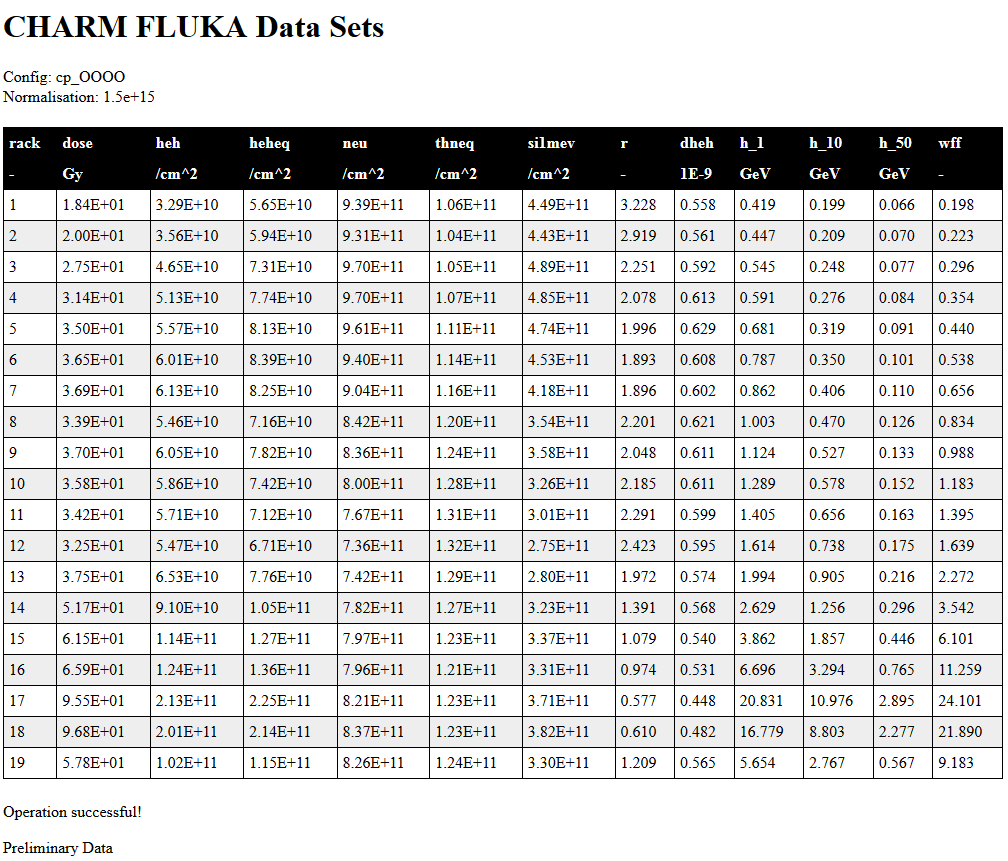
\includegraphics[width=\textwidth]{./images/fluka_datasets_example}}
	\caption{An example of a data-table from the FLUKA calculations for the CHARM test positions.}
	\label{fig:fluka_dataset}
\end{figure}

\begin{figure}[!ht]
	\centering
	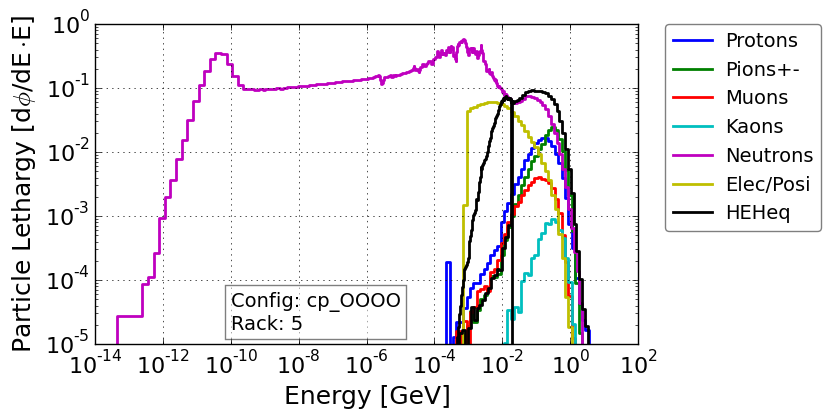
\includegraphics[scale=0.6]{./images/spectra_cp_OOOO_r5}
	\caption{An example plot of the radiation spectra at a test position for the facility configuration with the the copper target without shielding.}
	\label{fig:cpOOOO_spectra}
\end{figure}

\begin{figure}[!ht]
	\centering
	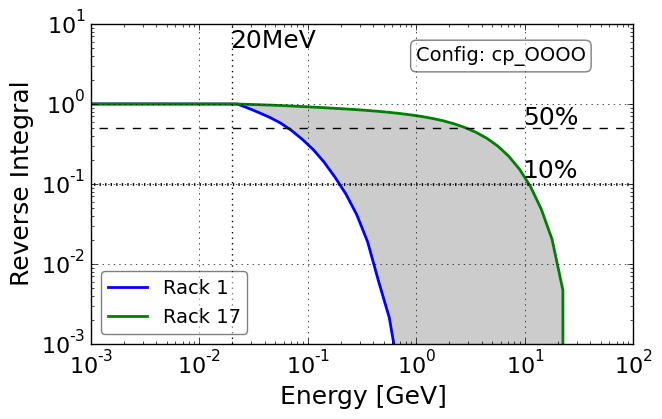
\includegraphics[scale=0.6]{./images/rev_spectra_cp_OOOO}
	\caption{A plot of the reverse integral spectra for the case with the copper target without shielding.}
	\label{fig:cpOOOO_rev_spectra}
\end{figure}

\begin{figure}[!ht]
	\centering
	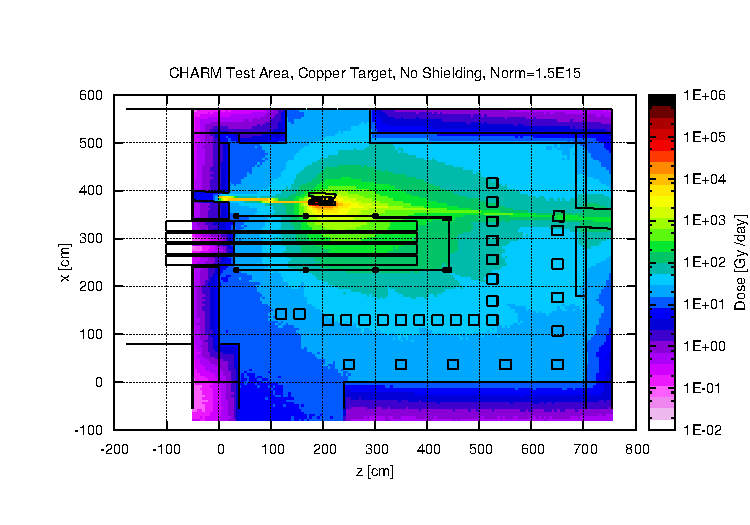
\includegraphics[width=\textwidth]{./images/dose_test_area_cpOOOO_norm}
	\caption{A plot of the dose per day inside the test area at beam height, normalised for the normal beam conditions.}
	\label{fig:cp_OOOO_dosemap}
\end{figure}

\clearpage
\section{Montrac Test Position}

MAYBE BETTER IN THE INTRODUCTION \\

Testing at the Montrac location is typically performed without the target, which means the radiation field is dominated by the primary beam. Therefore it is only suitable for tests requiring a mono-energetic proton beam of 24 GeV. However as the dose rate and particle fluence is high, it is a good place for dose testing, radiation damage to materials, and for detector calibration purposes. \\

The tests parameters are limited by the beam conditions, namely in the intensity and frequency of the spills, and the dimensions in the x and y plane. There are two main modes for the kind of beam sent to CHARM: target beam and blown-up beam conditions, shown in table X. These conditions can vary during operation, depending on the requirements for the various PS beam users. \\

% testing in mono-energetic protons
% dose, materials studies, calibration
% tests parameters restricted by the beam conditions (intensity, spill frequency, beam size)
% % 2 options: target beam (2.4cm^2), blown-up beam (8x12cm)
% % these conditions can vary during operation (FWHM, centre) 


Dose, HEH, 1MeV-eq n fluence in Si, beam size, gradients, peak values:
\begin{itemize}
	\item In-beam tests (normal beam)
	\item In-beam tests (blown-up beam)
	\item Tests with target
\end{itemize}

\begin{figure}[!ht]
	\centering
	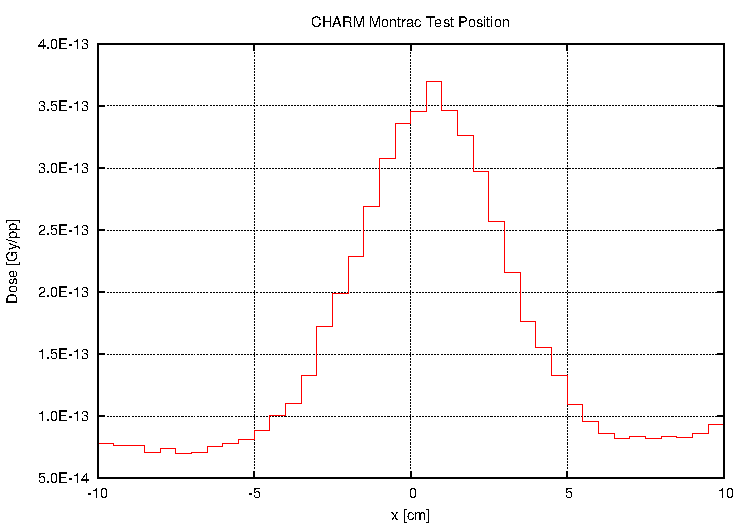
\includegraphics[width=0.45\textwidth]{./images/montrac_dose_1d_x}\quad
	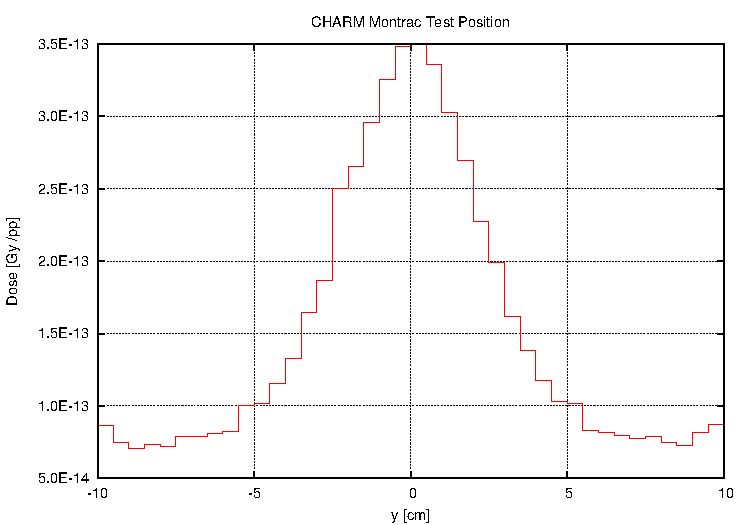
\includegraphics[width=0.45\textwidth]{./images/montrac_dose_1d_y}
	\caption{A plot of the dose profiles per proton at the Montrac test location (in beam).}
	\label{fig:montrac_cp_OOOO_dose}
\end{figure}

\begin{figure}[!ht]
	\centering
	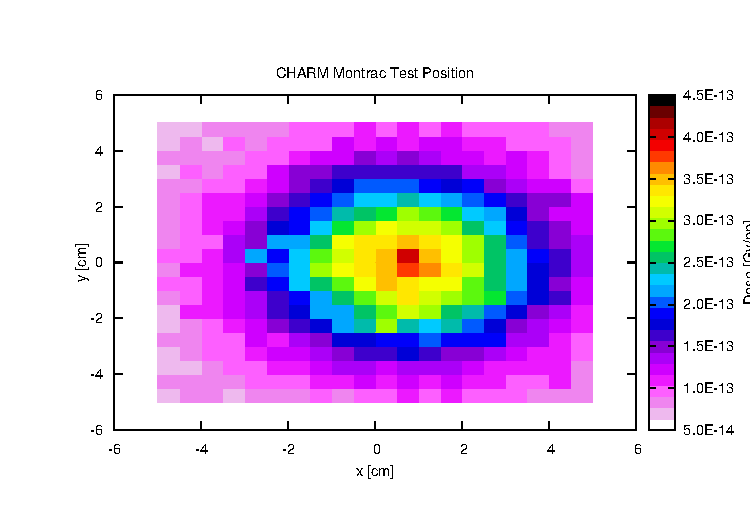
\includegraphics[width=0.7\textwidth]{./images/montrac_dose_2D}\
	\caption{A plot of the dose per proton in 2D at the Montrac test location (in beam).}
	\label{fig:montrac_cp_OOOO_dose_2D}
\end{figure}

\newpage
\section{Uncertainties}

There are a number of errors and uncertainties associated with the FLUKA calculations. The first main contributing factor is the accuracy of the geometry. This is in term of position of objects inside the main simulation geometry, materials and dimensions. Secondly there may be errors when comparing the calculations to tests made in the real facility due to positioning, and accurately the device was placed. There needs to be considerations for the test device itself, as the size of the sensitive volume may be large. These points are explored below with the aim of summarizing the various potential errors. \\

Gradients (in beam as well as test positions) \\

\end{document}